\chapter{Spettroscopia}
%\epigraph{Persino gli spettri scopano.}{Anonimo}
Tramite la fotometria abbiamo appreso come misurare la radiazione elettromagnetica in bande larghe di \SI{1500}{\angstrom} o strette di \SI{150}{\angstrom}. Questo ci permette di risalire alle proprietà generali della sorgente che la emette, come la temperatura e la distanza. Tuttavia, come abbiamo visto, tra le sorgenti e i nostri strumenti si trovano oggetti materiali che la luce deve attraversare per raggiungerci.

Proviamo per un attimo a fare un ragionamento al contrario: immaginiamo di avere una sorgente di cui conosciamo tutte le caratteristiche principali---ad esempio proprio un corpo nero---e interponiamo, tra noi e la sorgente, della materia non completamente opaca e non completamente ionizzata. Possiamo ad esempio confrontare la luce che arriva ai nostri strumenti con la distribuzione nota prodotta dal corpo nero, al fine capire come la radiazione interagisce con la materia e dedurre da ciò le sue proprietà.
\section{Spettrografi}\label{s:spettrografi}
    Per cominciare, per poter misurare la radiazione in modo più dettagliato servono strumenti appositi. Per gli studi di fotometria infatti possiamo ``accontentarci'' di fotografare una stella con un sensore che sia sensibile, più o meno allo stesso modo, a tutte le lunghezze d'onda cambiando di volta in volta i filtri a banda larga o stretta per scegliere quali fotoni far passare. Se invece vogliamo fare uno studio più dettagliato a banda ``strettissima'' dovremmo cambiare uno alla volta decine di migliaia di filtri---uno per ciascun intervallo di ampiezza $\dd{\nu}$ o $\dd{\lambda}$---a meno che non decidiamo di ricorrere a metodi più specializzati.

    Gli strumenti utilizzati in spettroscopia si chiamano \emph{spettrografi} e si basano sulla capacità di alcuni apparati di \emph{disperdere} la luce, ovvero separarla nei colori che la compongono, come prismi e reticoli di diffrazione. I primi deviano la luce incidente di un angolo che dipende dalla lunghezza d'onda, permettendo di separare spazialmente fasci di luce di colori diversi; i reticoli invece sfruttano i fenomeni di interferenza tra fasci di luce che incidono sul reticolo formando picchi di interferenza costruttiva ad angoli che dipendono dalla lunghezza d'onda.

    Dopo aver separato i colori di un fascio di luce tramite un \emph{dispersore}, possiamo intercettare i fasci con uno schermo o un sensore e fare una ``foto'': quello che si vedrà sarà una collezione di righe più o meno large e separate tra loro. Introduciamo quindi dei parametri che ci permettano di qualificare le proprietà di uno spettrografo: il \emph{potere dispersivo} e il \emph{potere risolutivo}.
    
    Il potere dispersivo è la capacità dello spettrografo di disperdere, ovvero separare spazialmente, le lunghezze d'onda. Maggiore è il potere dispersivo più sarà facile distinguere righe vicine nello spettro in quanto vengono separate maggiormente sullo schermo. Il potere risolutivo invece è, come per i telescopi, la capacità dello strumento di risolvere due picchi distinti vicini tra loro. Infatti per la diffrazione dovuta alle dimensioni finite delgli strumenti\footnote{Questa è una caratteristica legata puramente alla geometria degli strumenti che non c'entra con l'allargamento di riga dovuto alle relazioni di indeterminazione [VEDI par giusto].} le bande di emissione hanno uno spessore finito e la risoluzione di due picchi vicini è un problema del tutto analogo alla risoluzione dei dischi di Airy di due stelle. Possiamo quindi adottare il criterio di Rayleigh e affermare che due picchi sono distinguibili se la loro \FWHM\ è minore della distanza tra le due righe. Definiamo il potere risolutivo $R$ numericamente come
    \begin{equation}
        R = \frac{\lambda}{\Delta\lambda}
        \mycomma
    \end{equation}
    che in ambito di spettroscopia astronomica assume valori di \num{e5}--\num{e6}.

    Avere un potere risolutivo e dispersivo elevato non è importante solo per distinguere picchi vicini: spesso può essere utile usare uno spettrografo per determinare lo spostamento di una riga a causa dell'effetto doppler. Tuttavia tale spostamento può risultare troppo piccolo per essere rivelato consistentemente, come nei casi in cui la lunghezza d'onda originale $\lambda$ e quella spostata $\lambda + \dd{\lambda}$ ricadono nello stesso pixel del sensore.

    Per aumentare il potere dispersivo dello strumento, la fortuna---o meglio l'ottica---è apparentemente dalla nostra parte se usiamo un reticolo di diffrazione. I reticoli infatti producono diverse figure di interferenza a \emph{ordini} diversi e le figure di ordine maggiore risultano più disperse. Tuttavia a un aumento di separazione spaziale in questo caso corrisponde una diminuzione della luminosità delle righe e una minore nitidezza dell'immagine, dal momento che la maggior parte della luce convoglia nella figura al primo ordine.
    
    Per risolvere questo problema è stato inventato un nuovo tipo di reticolo di diffrazione in riflessione, costituito da un blocco di vetro plasmato a gradini con precisione micrometrica e rivestito con uno strato riflettetnte come esemplificato in \figref{fig:grating-spectrographer}. In questo tipo di spettrografo l'ordine più luminoso è anche quello con la maggiore dispersione, risultando molto più efficiente e preciso del reticolo in trasmissione.
    \begin{figure}
        \centering
        %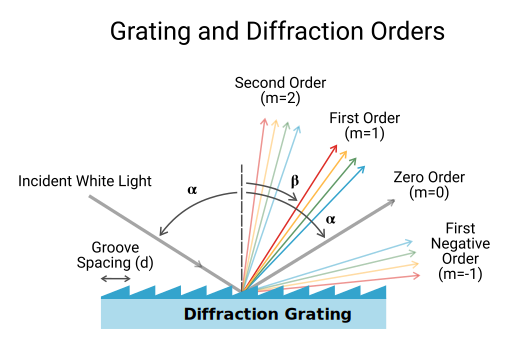
\includegraphics[width=\imagebig, trim={0 0 0 80pt}, clip]{images/spettroscopia/spectrograph.svg}
        \caption{Dispersore in riflessione di uno spettrografo.}
        \label{fig:grating-spectrographer}
    \end{figure}

\section{Assorbimento ed emissione}
    La materia che la radiazione elettromagnetica attraversa dopo aver lasciato la stella è di vario tipo: polveri e grani, gas ionizzati, plasmi, e le stesse atmosfere della stella e del nostro pianeta, ammesso che i nostri strumenti non si trovino nello spazio.

    I fenomeni di interazione che possono verificarsi sono prevalentemente di tre tipi:
    \begin{enumerate}[label=\ding{70}]
        \item \emph{Vero assorbimento}, quando il fotone di energia $E = h\nu$ viene completamente assorbito da un atomo che si ionizza. L'energia del fotone si trasforma in energia cinetica dell'elettrone, ovvero energia termodinamica;
        \item \emph{Vera emissione}, quando un atomo eccitato da urti anelastici---detti anche \emph{collisoni}---con altri atomi emette radiazione diseccitandosi. L'energia termodinamica viene quindi trasformata in luce;
        \item \emph{Diffusione e transizioni}, fenomeni elastici o anelastici in cui un fotone interagisce con un elettrone libero o legato, cede ad esso energia e viene diffuso cambiando lunghezza d'onda.
    \end{enumerate}
    Questi sono fenomeni che possono alterare in aspetto e in intensità lo spettro incidente in uno strato di materiale. Vediamoli più nel dettaglio.
    \subsection{Vero assorbimento}
        Il vero assorbimento si ha quando un fotone ha un'energia $E = h\nu$ maggiore dell'energia di (prima) ionizzazione $E_0$ dell'atomo colpito. In tal caso il quanto di luce sarà del tutto assorbito dall'elettrone, che sarà a sua volta sbalzato fuori dall'atomo con un'energia cinetica $K_\text{e}$ pari alla differenza tra energia del fotone ed energia di ionizzazione:
        \begin{equation*}
            K_\text{e} = \frac{1}{2} m_\text{e} v^2 = h\nu - E_0 > 0
            \myperiod
        \end{equation*}
        
        Come è noto dalla termodinamica, l'energia cinetica totale del gas di elettroni ionizzati è legata alla velocità quadratica media $\myavg{v^2}$ da
        \begin{equation}
            K = \frac{1}{2}m_\text{e}\myavg{v^2} = \frac{3}{2} N k_\text{B} T
            \mycomma
        \end{equation}
        essendo $N$ il numero di elettroni e $k_\text{B} = \SI{1.380e-23}{\joule\kelvin^{-1}}$ la costante di Bnuoltzmann. Possiamo quindi immaginare di trattare il gas di elettroni a temperatura $T$ come un corpo nero che emette un nuovo campo di radiazione che ha l'andamento di una planckiana corrispondente alla temperatura $T$, in generale diversa dallo spettro incidente che potrebbe avere una forma qualsiasi.\footnote{Ovviamente la distribuzione non può essere effettivamente \emph{qualsiasi}: lo spettro deve contenere fotoni di energia sufficiente a ionizzare il materiale.}
    \subsection{Vera emissione}
        A volte può succedere che due atomi collidano anelasticamente, ma l'energia non conservata dall'urto\footnote{È importante ricordare che \textsc{non} si tratta di urti classici ma di fenomeni di meccanica quantistica ben più complicati. Nel nostro caso una trattazione semi-classica è sufficiente a comprendere il fenomeno a grandi linee.} non può certo sparire nel nulla: in questi casi essa viene ``presa in prestito'' da un elettrone esterno di uno dei due atomi che passa a uno stato eccitato. Tuttavia l'elettrone non può rimanere indefinitamente in uno stato a energia superiore al minimo consentito e decadrà spontaneamente al suo \emph{ground state} emettendo un fotone che ha energia $E = h\nu$ esattamente pari alla differenza di energia $\Delta E$ tra i due livelli energetici occupati dall'elettrone.

        Questo tipo di emissione viene rivelata come una \emph{riga} 
        %\cfr{s:spettrografi}
        a una o più lunghezze d'onda ben precise corrispondenti proprio alle frequenze $\nu$, che sono determinate dal materiale: le differenze tra i vari livelli energetici cambiano da atomo ad atomo e da molecola a molecola, quindi le righe emesse da materiali diversi saranno in generale diverse. Se allora osserviamo una nube che emette per collisioni, possiamo confrontare le righe che riveliamo con gli spettri realizzati in laboratorio fino a trovare una corrispondenza e ``indovinare'' la composizione chimica della nube.
    \subsection{Scattering e transizioni}
        I fenomeni di scattering 
\section{Equazione del trasporto radiativo}
    Come abbiamo visto, esistono molteplici fenomeni che possono alterare in contemporanea lo spettro della radiazione che attraversa un materiale. e in Astrofisica si tende a raggruppare tutti questi fenomeni per lunghezza d'onda piuttosto che per tipo. Se nel nostro spettro è presente una riga in assorbimento non siamo in grado di sapere a priori quale fenomento ha fatto sparire tale riga, quindi piuttosto andiamo a vedere come l'intensità della radiazione varia al variare della lunghezza d'onda. Costruiamo adesso un'equazione che ci permetta di formalizzare quanto detto fin'ora.
    \subsection{Estinzione e opacità}
        Come per la fotometria, introduciamo anche in questo caso il \emph{coefficietne di estinzione} $\kappa_\nu$ tale che $\dd{I_\nu} = -\rho\kappa_{\nu}I_{\nu}\dd{x}$. Si definisce inoltre il \emph{coefficiente di opacità} come
        \begin{equation}
            \chi_\nu = \rho\kappa_\nu
            \mycomma
        \end{equation}
        dove la densità di massa $\rho$ del mezzo può essere sostituita dalla densità di grani $n$. Una proprietà importante del coefficiente di estinzione è che esso rappresenta una sorta di probabilità di interazione del fotone con la materia, per cui il suo reciproco rappresenta il libero cammino medio del fotone.

        Questa proprietà è strettamente legata al concetto di \emph{sezione d'urto}, ovvero la probabilità che due particelle interagiscono. Per la nostra trattazione assumeremo che la sezione d'urto $\sigma_{\nu}$---che è analoga a una superficie e quindi si misura in \unit{m^2}---sia sempre molto piccola rispetto alla distanza media tra le particelle:
        \begin{equation*}
            \sqrt{\sigma} \ll d \sim \frac{1}{\sqrt[3]{n}}
            \myperiod
        \end{equation*}
        Di conseguenza se $\kappa_\nu$ rappresenta una probabilità di interazione, come $\sigma$, possiamo scrivere il coefficiente di opacità come $\chi_\nu = n\kappa_\nu \approx n\sigma_{\nu}$. Se rimuovessimo l'ipotesi di sezioni d'urto piccole sarebbe impossibile fare questa considerazione perché una particella con sezione d'urto molto grande metterebbe in ombra tutte quelle che la seguono lungo il tragitto del fotone e bisognerebbe tenere conto di questo effeto. La possibilità di mettere in relazione $\kappa_\nu$, $\sigma_\nu$ ed $n$ ci permette di determinare la numerosità delle particelle, che in Astrofisica prende il nome di \emph{abbondanza}.

        Un'altra ipotesi importante che stiamo facendo implicitamente è che il mezzo sia isotropo, ovvero che si comporti allo stesso modo in tutte le direzioni, cosa che naturalmente non è in generale vera dal momento che i grani non hanno forma sferica e il mezzo interstellare potrebbe interagire coi campi elettromagnetici polarizzandosi e cambiando le sue proprietà.
    \subsection{Emissività e sorgente}
        Abbiamo visto che alcuni fenomeni come la vera emissione possono portare il materiale a introdurre nuovi fotoni nel campo di radiazione comportandosi a sua volta come sorgente. Introduciamo quindi un coefficiente macroscopico $\eta_\nu$ che prende il nome di \emph{coefficiente di emissività} e in modo analogo all'estinzione dà un contributo
        \begin{equation}
            \label{eq:emissività}
            \dd{I_\nu} = \eta_{\nu}\dd{x}
        \end{equation}
        che però è indipendente dall'intensità specifica $I_\nu$ incidente. Se sommiamo il contributo dell'estinzione a quello dell'emissione otteniamo quindi
        \begin{equation*}
            \dd{I_\nu} = \pqty{\eta_\nu - \chi_\nu I_\nu}\dd{x}
            \mycomma   
        \end{equation*}
        che, introducendo la funzione \emph{sorgente} $S_\nu$ tale che $S_\nu\chi_\nu = \eta_\nu$, può essere riscritta come:
        \begin{equation}
            \label{eq:trasporto-radiativo}
            \dv{I_\nu}{x} = \chi_{\nu}\pqty{S_{\nu} - I_{\nu}}
            \myperiod
        \end{equation}
        Questa equazione prende il nome di \emph{equazione completa del trasferimento} e gioca un ruolo essenziale nello studio degli astri. L'equazione \eqref{eq:trasporto-radiativo} è più spesso detta \emph{equazione del trasporto radiativo} anche se non vi è alcun effettivo movimento di materia; quest'ultimo nome è utilizzato solo in Astrofisica.
\section{Soluzione dell'equazione del trasporto}
    L'equazione \eqref{eq:trasporto-radiativo} è in via di massima impossibile da risolvere analiticamente ma può essere risolta numericamente. Mettiamoci quindi in un contesto di nostro interesse ed effettuiamo alcune ulteriori semplificazioni.

    Naturalmente, volendo prevalentemente applicare questa equazione allo studio delle stelle, in tutti casi dovremo tenere conto del fatto che la radiazione prodotta nel nucleo di una stella deve attraversare l'atmosfera stellare prima di giungere nel mezzo interstellare. È quindi di nostro interesse trovare una soluzione ``generale'' per l'equazione \eqref{eq:trasporto-radiativo} in un contesto accessibile, come l'atmosfera del nostro Sole, per poi applicare il risultato alle stelle simili.

    Come abbiamo fatto per l'estinzione atmosferica \cfr{ss:estinzione-atmosferica}, supponiamo che l'atmosfera stellare, molto sottile rispetto al diametro della stella, sia suddivisibile in tanti gusci sferici sovrapposti di spessore $\dd{r}$. Se consideriamo un elemento di superficie sferica, la luce che lo attraversa viaggia in tutte le direzioni, quindi in particolare viaggia nella nostra direzione $\dd{s}$ che forma un angolo $\vartheta$ con la normale all'elemento superficiale.
    Lungo questa direzione, la \eqref{eq:trasporto-radiativo} si scrive
    \begin{equation}
        \label{eq:tr-rad-s}
        \dv{I_\nu}{s} = \chi_{\nu}\pqty{S_{\nu} - I_{\nu}}
        \myperiod
    \end{equation}
    Lo spostamento elementare $\dd{r}$ in questo caso è pari a $\dd{r} = - \cos\vartheta\dd{s}$. Il segno meno è dovuto al fatto che mentre la luce va dall'interno della stella verso l'esterno, noi effettuiamo la nostra misura a partire dall'esterno e integrando verso l'interno, allontanandoci dal nostro punto di vista; il verso di percorrenza della traiettoria è quindi opposto. Sostituendo questa relazione nella \eqref{eq:tr-rad-s}, invertendo e ponendo $\mu = \cos\vartheta$, otteniamo al primo membro:
    \begin{equation*} 
        \dv{I_\nu}{r}
        = -\frac{1}{\cos\vartheta} \dv{I_\nu}{s}
        \implies \dv{I_\nu}{s}
        = -\mu\dv{I_\nu}{r}
        \mycomma
    \end{equation*}
    che, inserito nella \eqref{eq:tr-rad-s}, diventa:
    \begin{equation}
        \label{eq:tr-rad-mu}
        -\mu\dv{I_\nu}{r} = \chi_{\nu}\pqty{S_{\nu} - I_{\nu}}
        \myperiod
    \end{equation}

    Se adesso riprendiamo la profondità ottica dalla definizione \eqref{eq:profondità-ottica} si ha $\dd{\tau_\nu} = \kappa_\nu \rho \dd{r} = \chi_\nu\dd{r}$. Se dividiamo la \eqref{eq:tr-rad-mu} per $\chi_\nu$ otteniamo
    \begin{equation*}
        -\mu\frac{1}{\chi_\nu} \dv{I_\nu}{r}
        = -\mu \dv{I_\nu}{\tau_\nu}
        = S_{\nu} - I_{\nu}
        \mycomma
    \end{equation*}
    e cambiando di segno
    \begin{equation}
        \label{eq:tr-rad-tau}
        \mu \dv{I_\nu}{\tau_\nu}
        = I_{\nu} - S_{\nu} 
        \myperiod
    \end{equation}

    Quest'ultima equazione può essere facilmente risolta nel caso $\mu = 1$, ovvero quando la superficie stellare è perpendicolare alla linea di vista. Moltiplicando la \eqref{eq:tr-rad-tau} per $e^{-\tau_\nu}$  abbiamo
    \begin{equation*}
        e^{-\tau_\nu} \dv{I_\nu}{\tau_\nu}
        = e^{-\tau_\nu}\pqty{I_{\nu} - S_{\nu}}
        \iff e^{-\tau_\nu} \dv{I_\nu}{\tau_\nu} - e^{-\tau_\nu}I_{\nu}
        = -e^{-\tau_\nu} S_{\nu}
    \end{equation*}
    e, applicando la regola di derivazione del prodotto,
    \begin{equation*}
        \dv{\tau_\nu}\pqty{e^{-\tau_\nu}I_{\nu}} = -e^{-\tau_\nu} S_{\nu}
        \myperiod
    \end{equation*}
    A questo punto possiamo integrare nella variabile $\tau_\nu$ da un valore $\tau_\nu^2$ a $\tau_\nu^1$, ponendo $I_{\nu}^2 = I_{\nu}\pqty{\tau_\nu^2}$ e $I_{\nu}^1 = I_{\nu}\pqty{\tau_\nu^1}$:
    \begin{equation*}
        e^{-\tau_\nu^1}I_{\nu}^1 - e^{-\tau_\nu^2}I_{\nu}^2
        = -\int_{\tau_\nu^2}^{\tau_\nu^1} e^{-\tau_\nu} S_{\nu}\pqty{\tau_\nu} \dd{\tau_\nu}
        = \int_{\tau_\nu^1}^{\tau_\nu^2} e^{-\tau_\nu} S_{\nu}\pqty{\tau_\nu} \dd{\tau_\nu}
        \myperiod
    \end{equation*}
    Nel caso particolare $\tau_\nu^1 = 0$ e $\tau_\nu^2 = \tau_\nu$, possiamo scrivere:
    \begin{equation}
        \label{eq:tr-rad-int}
        I_\nu\pqty{0} = e^{-\tau_\nu}I_{\nu}\pqty{\tau_\nu} + \int_0^{\tau_\nu} e^{-\tau_{\nu}'} S_{\nu}\pqty{\tau_{\nu}'} \dd{\tau_{\nu}'}
        \mycomma
    \end{equation}
    dove $I_\nu\pqty{0}$ è l'intensità specifica totale emergente dalla somma dei contributi di tutti gli strati: i fotoni che partono dallo strato di profondità ottica $\tau_\nu$ incidono sullo strato successivo, essi vengono attenuati esponenzialmente e ad essi si aggiungono i fotoni introdotti dall'emissione negli strati precedenti. Si prosegue così fino ad arrivare fuori dall'atmosfera, il punto $\tau_\nu = 0$, da cui noi facciamo invece cominciare l'integrazione.

    L'integrale che compare nella \eqref{eq:tr-rad-int} può essere risolto numericamente tenendo conto del fatto che se la profonodità ottica del mezzo è particolarmente elevata possiamo fermarci quando i contributi sono pressoché nulli.

    Un'utile approssimazione che viene fatta in Astrofisica è quella di supporre che la sorgente della radiazione abbia spessore infinito, coerentemente col fatto che lo spessore delle atmosfere stellari è estremamente ridotto se confrontato al diametro della stella: ciò equivale matematicamente a fare il limite della \eqref{eq:tr-rad-int} per $\tau_\nu \to +\infty$. Se supponiamo che
    \begin{equation*}
        \lim_{\tau_\nu \to +\infty} e^{-\tau_\nu}I_{\nu}\pqty{\tau_\nu} = 0
        \mycomma
    \end{equation*}
    che è lecito in quanto una sorgente reale non può emettere radiaizone infinita, la \eqref{eq:tr-rad-int} diventa
    \begin{equation}
        \label{eq:tr-rad-lim}
        I_\nu\pqty{0} = \int_0^{+\infty} e^{-\tau_{\nu}'} S_{\nu}\pqty{\tau_{\nu}'} \dd{\tau_{\nu}'}
        \myperiod
    \end{equation}
    Il significato fisico di questo risultato è che la radiazione che incide sul primo strato di atmosfera sostanzialmente non dà nessun contributo alla radiazione che osserviamo al di fuori di essa: all'esterno dell'atmosfera, dove al solito $\tau_\nu = 0$, giungono solo i contributi in emissione dovuti all'atmosfera stessa. Questo modello descrive sufficientemente bene i casi reali in cui si ha $\tau_\nu \gg 1$, ovvero quando la materia è particolamrnete densa e la probabilità di interazione fotone--materia è circa uguale a \num{1}. In questi casi si dice che il plasma è \emph{otticamente spesso} e quindi opaco alla frequenza $\nu$.

    Nel caso opposto in cui si ha $\tau_\nu \ll 1$ l'approssimazione non vale più. Per $\tau_\nu \to 0$, l'esponenziale tende a \num{1} e la \eqref{eq:tr-rad-int} si semplifica in
    \begin{equation*}
        I_\nu\pqty{0} = I_{\nu}\pqty{\tau_\nu} + \int_0^{\tau_\nu} e^{-\tau_{\nu}'} S_{\nu}\pqty{\tau_{\nu}'} \dd{\tau_{\nu}'}
        \myperiod
    \end{equation*}
    Questo significa che la radiazione incidente non viene estinta e ad essa si aggiungono i contributi in emissione di ogni strato. In questi casi si parla di plasma \emph{otticamente sottile}.

    Se ci soffermiamo un attimo a osservare la \eqref{eq:tr-rad-lim} notiamo che formalmente ricorda una trasformata integrale, in particolare la trasformata di Laplace. Data una funzione $f$ della variabile $t$, la sua trasformata di Laplace unilatera\footnote{Ovvero integrando su $\left[0,+\infty\right[$ piuttosto che su $\left]-\infty,+\infty\right[$.} si scrive:
    \begin{equation*}
        \mcL\qty{f}\pqty{s} = \int_0^{+\infty} e^{-st} f\pqty{t} \dd{t}
        \myperiod
    \end{equation*}
    Quindi l'intensità $I_\nu$ calcolata nel punto $\tau_\nu = 0$ corrisponde alla trasformata di Laplace della funzione sorgente $S_\nu$,
    \begin{equation*}
        \bqty{I_{\nu}\pqty{0}}\pqty{s} = \int_0^{+\infty} e^{-s\tau_\nu} S_\nu\pqty{\tau_\nu} \dd{\tau_\nu}
        \mycomma
    \end{equation*}
    calcolata per $s = 1$.
\section{Spettri stellari}
    Un problema non indifferente dell'equazione del trasporto è che per poterla effettivamente risolvere sarebbe necessario conoscere le quantità $S_\nu$, $\tau_\nu$, $\chi_\nu$ \myetc, conoscenza che all'astronomo manca. Come già detto altre volte, noi possiamo misurare solo il ``risutlato finale'' dell'integrazione e non gli andamenti delle funzioni punto per punto. Quello che possiamo fare quindi è osservare gli spettri misurati e invertire ``a tentativi'' le relazioni per trovare delle funzioni che spieghino i dati.

    Osserviamo alcuni spettri [inserire foto fantasmini paurosi]
    

\section{Equazione di Saha??}